\documentclass[10pt,a4paper]{article}
\usepackage[UTF8,fontset = windows]{ctex}
\setCJKmainfont[BoldFont=黑体,ItalicFont=楷体]{华文中宋}
\usepackage{amssymb,amsmath,amsfonts,amsthm,mathrsfs,dsfont,graphicx}
\usepackage{ifthen,indentfirst,enumerate,color,titletoc}
\usepackage{tikz}
\usepackage{makecell}
\usepackage{longtable}
%\usepackage{mathptmx}

\usetikzlibrary{arrows,calc,intersections,patterns,decorations.pathreplacing}
\usepackage[bf,small,indentafter,pagestyles]{titlesec}
\usepackage[top=1in, bottom=1in,left=0.8in,right=0.8in]{geometry}
\renewcommand{\baselinestretch}{1.65}
\newtheorem{defi}{定义~}
\newtheorem{eg}{例~}
\newtheorem{ex}{~}
\newtheorem{rem}{注~}
\newtheorem{thm}{定理~}
\newtheorem{coro}{推论~}
\newtheorem{axiom}{公理~}
\newtheorem{prop}{性质~}
\newcommand{\blank}[1]{\underline{\hbox to #1pt{}}}
\newcommand{\bracket}[1]{(\hbox to #1pt{})}
\newcommand{\onech}[4]{\par\begin{tabular}{p{.9\textwidth}}
A.~#1\\
B.~#2\\
C.~#3\\
D.~#4
\end{tabular}}
\newcommand{\twoch}[4]{\par\begin{tabular}{p{.46\textwidth}p{.46\textwidth}}
A.~#1& B.~#2\\
C.~#3& D.~#4
\end{tabular}}
\newcommand{\vartwoch}[4]{\par\begin{tabular}{p{.46\textwidth}p{.46\textwidth}}
(1)~#1& (2)~#2\\
(3)~#3& (4)~#4
\end{tabular}}
\newcommand{\fourch}[4]{\par\begin{tabular}{p{.23\textwidth}p{.23\textwidth}p{.23\textwidth}p{.23\textwidth}}
A.~#1 &B.~#2& C.~#3& D.~#4
\end{tabular}}
\newcommand{\varfourch}[4]{\par\begin{tabular}{p{.23\textwidth}p{.23\textwidth}p{.23\textwidth}p{.23\textwidth}}
(1)~#1 &(2)~#2& (3)~#3& (4)~#4
\end{tabular}}
\begin{document}
\begin{enumerate}[1.]

\item 已知$\sin x=-\dfrac 13$($\pi <x<\dfrac{3\pi }2$), 用反正弦形式表示$x$.\\
解答在这里  因为$\sin (\pi -x)=\sin x=-\dfrac 13$, 且由$\pi <x<\dfrac{3\pi }2$知, $-\dfrac{\pi }2<\pi -x<0$,
所以$\pi -x=\arcsin (-\dfrac 13)=-\arcsin \dfrac 13$, 于是$x=\pi +\arcsin \dfrac 13$.
\item 若$\cos x=\dfrac 13$($-\dfrac{\pi }2<x<0$), 用反余弦形式表示$x$.\\
解答在这里  因为$\cos (-x)=\cos x=\dfrac 13$, 且由$-\dfrac{\pi }2<x<0$知, $0<-x<\dfrac{\pi }2$,
所以$-x=\arccos \dfrac 13$, 故$x=-\arccos \dfrac 13$.
\item 求值: $\tan [\dfrac 12\arcsin (\dfrac{-2\sqrt 6}5)]$.\\
解答在这里 令$\alpha =\arcsin (\dfrac{-2\sqrt 6}5)$, 则$\sin \alpha =\dfrac{-2\sqrt 6}5$, $\alpha \in (-\dfrac{\pi }2,0)$, 于是$\cos \alpha =\dfrac 15$.
所以原式$=\tan \dfrac\alpha 2=\dfrac{1-\cos \alpha }{\sin \alpha }=\dfrac{1-\dfrac 15}{-\dfrac {2\sqrt 6}5}=-\dfrac{\sqrt 6}3$.
\item 求值: $\cos [\arctan \dfrac 34+\arccos (-\dfrac 23)]$.
解答在这里 令$\alpha =\arctan \dfrac 34$, 则$\tan \alpha =\dfrac 34$, $\alpha \in (0,\dfrac{\pi }2)$, 于是$\sin \alpha =\dfrac 35$, $\cos \alpha =\dfrac 45$. 又$\beta =\arccos (-\dfrac 23)$, 则$\cos \beta =-\dfrac 23$, $\beta \in (\dfrac{\pi }2,\pi)$, 于是$\sin \beta =\dfrac{\sqrt 5}3$.
所以原式$=\cos (\alpha +\beta)=\cos \alpha \cos \beta -\sin \alpha \sin \beta =\dfrac 45\times (-\dfrac 23)-\dfrac 35\times \dfrac{\sqrt 5}3=-\dfrac {8+3\sqrt 5}{15}$.
\item 求值: $\arcsin (\sin 2)$.\\
解答在这里 (1)因为$\sin 2=\sin (\pi -2)$, 且$\pi -2\in [-\dfrac{\pi }2,\dfrac{\pi }2]$,
所以原式$=\arcsin [\sin (\pi -2)]=\pi -2$.
\item 求值: $\arccos (\cos \dfrac 65\pi)$.\\
解答在这里 因为$\cos \dfrac 65\pi =\cos \dfrac 45\pi$, 且$\dfrac 45\pi \in [0,\pi]$, 所以原式$=\arccos (\cos \dfrac 45\pi)=\dfrac 45\pi$.
\item 求值: $\arctan (\cot \sqrt 3)$.\\
解答在这里 因为$\cot \sqrt 3=\tan (\dfrac{\pi }2-\sqrt 3)$, 且$\dfrac{\pi }2-\sqrt 3\in (-\dfrac{\pi }2,\dfrac{\pi }2)$,
所以原式$=\arctan [\tan (\dfrac{\pi }2-\sqrt 3)]=\dfrac{\pi }2-\sqrt 3$.
\item 求值: $\mathrm{arccot} (-\cot \dfrac{\pi }7)$.
解答在这里 因为$-\cot \dfrac{\pi }7=\cot (-\dfrac{\pi }7)=\cot [\pi +(-\dfrac{\pi }7)]=\cot \dfrac 67\pi$, 且$\dfrac 67\pi \in (0,\pi)$, 所以原式$=\mathrm{arccot} (\cot \dfrac 67\pi)=\dfrac 67\pi$.
\item 若$|x|\le 1$, 求证: $\arcsin x+\arccos x=\dfrac{\pi }2$.\\
解答在这里 证法一  因为$\sin (\dfrac{\pi }2-\arccos x)=\cos (\arccos x)=x$, 其中$-1\le x\le 1$,
又由$\arccos x\in [0,\pi]$, 得$(\dfrac{\pi }2-\arccos x)\in [-\dfrac{\pi }2,\dfrac{\pi }2]$,
所以根据反正弦函数的定义, 得$\dfrac{\pi }2-\arccos x=\arcsin x$, 即$\arcsin x+\arccos x=\dfrac{\pi }2$.\\
证法二  设$\arcsin x=\alpha$, 则$\sin \alpha =x$, $\alpha \in [-\dfrac{\pi }2,\dfrac{\pi }2]$..
再设$\arccos x=\beta$, 则$\cos \beta =x$, $\beta \in [0,\pi]$.
因为$\sin \alpha =x$, $\sin (\dfrac{\pi }2-\beta)=\cos \beta =x$, 所以$\sin \alpha =\sin (\dfrac{\pi }2-\beta)$.
因为$-\dfrac{\pi }2\le \alpha \le \dfrac{\pi }2$, $-\dfrac{\pi }2\le \dfrac{\pi }2-\beta \le \dfrac{\pi }2$, 所以$\alpha =\dfrac{\pi }2-\beta$,
即$\alpha +\beta =\dfrac{\pi }2$, 所以$\arcsin x+\arccos x=\dfrac{\pi }2$.
\item 求证: $\arctan \dfrac 13+\arctan \dfrac 15+\arctan \dfrac 17+\arctan \dfrac 18=\dfrac{\pi }4$.\\
解答在这里  设$\alpha =\arctan \dfrac 13$, $\beta =\arctan \dfrac 15$, $\gamma =\arctan \dfrac 17$, $\delta =\arctan \dfrac 18$,
则$\tan \alpha =\dfrac 13$, $\tan \beta =\dfrac 15$, $\tan \gamma =\dfrac 17$, $\tan \delta =\dfrac 18$且$\alpha ,\beta ,\gamma ,\delta \in (0,\dfrac{\pi }4)$.
于是$\tan (\alpha +\beta)=\dfrac{\tan \alpha +\tan \beta }{1-\tan \alpha \tan \beta }=\dfrac{\dfrac 13+\dfrac 15}{1-\dfrac 13\times \dfrac 15}=\dfrac 47$,
$\tan (\gamma +\delta)=\dfrac{\tan \gamma +\tan \delta }{1-\tan \gamma \tan \delta }=\dfrac{\dfrac 17+\dfrac 18}{1-\dfrac 17\times \dfrac 18}=\dfrac 3{11}$.
所以$\tan (\alpha +\beta +\gamma +\delta)=\dfrac{\dfrac 47+\dfrac 3{11}}{1-\dfrac 47\times \dfrac 3{11}}=1$.
因为$0<\alpha +\beta +\gamma +\delta <\pi$, 所以$\alpha +\beta +\gamma +\delta =\dfrac{\pi }4$, 原命题得证.
\item 求满足不等式$\arcsin x<1$的$x$的取值范围.
解答在这里 由已知条件, 得$\begin{cases} -1\le x\le 1, \\ \arcsin x<\arcsin (\sin 1), \end{cases}$于是$\begin{cases} -1\le x\le 1, \\ x<\sin 1, \end{cases}$
所以$-1\le x<\sin 1$.
\item 求满足不等式$\arccos (2x^2-1)<\arccos x$的$x$的取值范围.
解答在这里 由已知条件, 得$\begin{cases} -1\le 2x^2-1\le 1, \\ -1\le x\le 1, \\ 2x^2-1>x, \end{cases}$即$\begin{cases} -1\le x\le 1, \\ 2x^2-x-1>0, \end{cases}$也即$\begin{cases} -1\le x\le 1, \\ x<-\dfrac 12x>1, \end{cases}$
所以$-1\le x<-\dfrac 12$.
\item 若$\pi \le \alpha \le \dfrac{3\pi }2$, 且$\sin \alpha =-\dfrac 14$, 则用反三角形式表示$\alpha$是\bracket{20}.
\fourch{$\pi -\arcsin \dfrac 14$}{$\pi +\arcsin \dfrac 14$}{$\dfrac{3\pi }2-\arcsin \dfrac 14$}{$\dfrac{3\pi }2+\arcsin \dfrac 14$}
\item 函数$y=\arcsin (\cot x)$的定义域是\bracket{20}.
\twoch{$[-1, 1]$}{$[k\pi +\dfrac{\pi }4,k\pi +\dfrac{3\pi }4]$($k\in \mathbf{Z}$)}{$[-\dfrac{\pi }4,\dfrac{\pi }4]$}{$[k\pi -\dfrac{\pi }4,k\pi +\dfrac{\pi }4]$($k\in \mathbf{Z}$)}
\item 函数$y=\sin (\arcsin x)$的图像是\bracket{20}.
\fourch{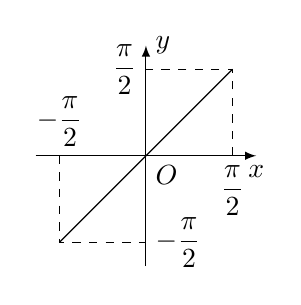
\begin{tikzpicture}[scale = 0.7,>=latex]
    \draw [->] (-2,0) -- (2,0) node [below] {$x$};
    \draw [->] (0,-2) -- (0,2) node [right] {$y$};
    \draw (0,0) node [below right] {$O$};
    \draw ({-pi/2},{-pi/2}) -- ({pi/2},{pi/2});
    \draw [dashed] ({pi/2},0) -- ({pi/2},{pi/2}) -- (0,{pi/2});
    \draw [dashed] ({-pi/2},0) -- ({-pi/2},{-pi/2}) -- (0,{-pi/2});
    \draw ({pi/2},0) node [below] {$\dfrac\pi 2$} ({-pi/2},0) node [above] {$-\dfrac\pi 2$} (0,{pi/2}) node [left] {$\dfrac\pi 2$} (0,{-pi/2}) node [right] {$-\dfrac\pi 2$};
\end{tikzpicture}}{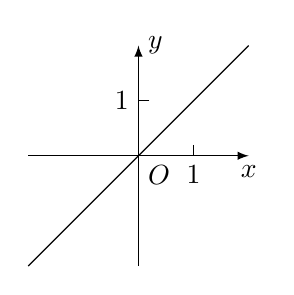
\begin{tikzpicture}[scale = 0.7,>=latex]
    \draw [->] (-2,0) -- (2,0) node [below] {$x$};
    \draw [->] (0,-2) -- (0,2) node [right] {$y$};
    \draw (0,0) node [below right] {$O$};
    \draw (-2,-2) -- (2,2);
    \draw (1,0.2) -- (1,0) node [below] {$1$} (0.2,1) -- (0,1) node [left] {$1$};
\end{tikzpicture}}{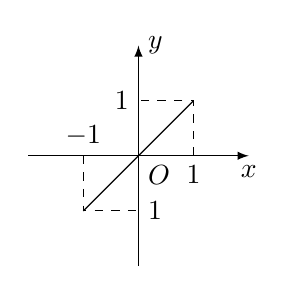
\begin{tikzpicture}[scale = 0.7,>=latex]
    \draw [->] (-2,0) -- (2,0) node [below] {$x$};
    \draw [->] (0,-2) -- (0,2) node [right] {$y$};
    \draw (0,0) node [below right] {$O$};
    \draw (-1,-1) -- (1,1);
    \draw [dashed] (1,0) -- (1,1) -- (0,1);
    \draw [dashed] (-1,0) -- (-1,-1) -- (0,-1);
    \draw (1,0) node [below] {$1$} (-1,0) node [above] {$-1$} (0,1) node [left] {$1$} (0,-1) node [right] {$1$};
\end{tikzpicture}}{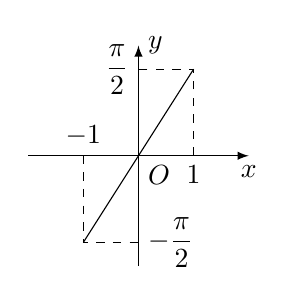
\begin{tikzpicture}[scale = 0.7,>=latex]
    \draw [->] (-2,0) -- (2,0) node [below] {$x$};
    \draw [->] (0,-2) -- (0,2) node [right] {$y$};
    \draw (0,0) node [below right] {$O$};
    \draw (-1,{-pi/2}) -- (1,{pi/2});
    \draw [dashed] (1,0) -- (1,{pi/2}) -- (0,{pi/2});
    \draw [dashed] (-1,0) -- (-1,{-pi/2}) -- (0,{-pi/2});
    \draw (1,0) node [below] {$1$} (-1,0) node [above] {$-1$} (0,{pi/2}) node [left] {$\dfrac\pi 2$} (0,{-pi/2}) node [right] {$-\dfrac\pi 2$};
\end{tikzpicture}}
\item 函数$f(x)=2\arcsin (x-1)$的反函数是\bracket{20}.
\twoch{$y=\dfrac 12\sin (x-1)$($-\dfrac{\pi }2<x<\dfrac{\pi }2$)}{$y=1+\sin \dfrac x2$($-\dfrac{\pi }2\le x\le \dfrac{\pi }2$)}{$y=1+\sin \dfrac x2$($-\pi \le x\le \pi$)}{$y=\sin (\dfrac x2+1)$($-\pi \le x\le \pi$)}
\item 函数$y=\arcsin (x^2-x)$为减函数的区间是\bracket{20}.
\fourch{$[-1, 1]$}{$[\dfrac 12,\dfrac 12(1+\sqrt 5)]$}{$(-\dfrac{\pi }4,+\infty)$}{$[\dfrac 12(1-\sqrt 5),\dfrac 12]$}
\item 若$0<a<1$, 则在$[0,2\pi]$内满足$\sin x\ge a$的$x$的取值范围是\bracket{20}.
\fourch{$[0,\arcsin a]$}{$[\arcsin a,\pi -\arcsin a]$}{$[\pi \arcsin a,\pi]$}{$[\arcsin a,\dfrac{\pi }2+\arcsin a]$}
\item 若$\dfrac{\pi }2\le x\le \dfrac{3\pi }2$, 则$\arcsin (\sin x)$的值等于\bracket{20}.
\fourch{$x$}{$\pi -x$}{$x-\pi$}{$x+\pi$}
\item 已知$\arcsin x\ge 1$, 则$x$的取值范围是\bracket{20}.
\fourch{$[0, 1]$}{$[0,\sin 1]$}{$[\sin 1,1]$}{$[-1, 1]$}
\item 若函数$y=\arcsin (\cos x)$的定义域是$(-\dfrac{\pi }3,\dfrac{2\pi }3)$, 则值域是\bracket{20}.
\fourch{$(-\dfrac{\pi }6,\dfrac{\pi }3]$}{$(-\dfrac{\pi }6,\dfrac{\pi }2]$}{$(\dfrac{\pi }6,\dfrac{\pi }2]$}{$[\dfrac{\pi }3,\dfrac{\pi }2]$}
\item 函数$y=\sqrt {\arcsin x}$的定义域为\blank{50}, 值域为\blank{50}.
\item 函数$y=\arcsin (\lg \dfrac x2)$的定义域为\blank{50}, 值域为\blank{50}.
\item 函数$y=\dfrac 12\arcsin \dfrac 1{x-2}$的定义域为\blank{50}, 值域为\blank{50}.
\item 函数$y=\arcsin (x-x^2)$的定义域为\blank{50}, 值域为\blank{50}.
\item 函数$f(x)=\log _2(\arcsin \dfrac x2)$的定义域为\blank{50}, 值域为\blank{50}.
\item 计算: $\arcsin [\sin (-\dfrac{5\pi }4)]=$\blank{50}.		
\item 计算: $\arcsin (\sin 3)=$\blank{50}.
\item 计算: $\arcsin (\cos 2)=$\blank{50}.
\item 计算: $\arcsin (\cos 5)=$\blank{50}.
\item 计算: $\arcsin (\sin \pi ^2)=$\blank{50}.
\item 求函数$y=(\arcsin x)^2-2\arcsin x-2$的最大值与最小值, 并求取得最大值、最小值时的$x$值.
\item 已知$a,b,c$依次为直角三角形的两直角边和斜边, 且满足$\arcsin \dfrac 1a+\arcsin \dfrac 1b=\dfrac{\pi }2$, 求证: $c=ab$.
\item 已知$\alpha =\dfrac{9\pi }8$, 求$\arcsin (\dfrac{\sin \alpha +\cos \alpha }{\sqrt 2})$的值.
\item 已知$\dfrac{\pi }4<\theta <\dfrac{5\pi }4$, 求证$\arcsin (\dfrac{\sin \theta +\cos \theta }{\sqrt 2})=\dfrac{3\pi }4-\theta$.
\item 求函数$f(x)=\sin (x-\dfrac{\pi }4)\cos (x+\dfrac{\pi }4), \ -\dfrac{\pi }4\le x\le \dfrac{\pi }4$的反函数.
\item 求函数$f(x)=\sin (x-\dfrac{\pi }4)\cos (x+\dfrac{\pi }4),\  \dfrac{\pi }4\le x\le \dfrac{\pi }2$的反函数.
\item 下列各式正确的是\bracket{20}.
\twoch{$\arcsin (-\dfrac{\pi }3)=-\dfrac{\sqrt 3}2$}{$\sin (\arcsin \dfrac{\pi }3)=\dfrac{\pi }3$}{$\arcsin (\sin \dfrac{5\pi }4)=\dfrac{\pi }4$}{$\sin [\arccos (-\dfrac{\sqrt 2}2)]=\dfrac{\sqrt 2}2$}
\item 在$[-1,\dfrac 32]$上与函数$y=x$相同的函数是\bracket{20}.
\fourch{$y=\arccos (\cos x)$}{$y=\arcsin (\sin x)$}{$y=\sin (\arcsin x)$}{$y=\cos (\arccos x)$}
\item 若$f(\cos x)=\dfrac x2$, $x\in [0,\pi]$, 则$f(-\dfrac 12)$等于\bracket{20}.
\fourch{$\cos \dfrac 12$}{$\dfrac{\pi }3$}{$\dfrac{\pi }4$}{$\dfrac{2\pi }3$}
\item 函数$y=\arccos (-x)$的图像与$y=\arccos x$的图像\bracket{20}.
\fourch{关于$x$轴对称}{关于$y$轴对称}{关于原点对称}{关于直线$y=x$对称}
\item 函数$y=\arccos (x^2-2x)$为减函数的区间是\bracket{20}.
\fourch{$[1,+\infty]$}{$[-1,1+\sqrt 2]$}{$[1-\sqrt 2,1+\sqrt 2]$}{$[1,1+\sqrt 2]$}
\item 函数$y=\sqrt {\arccos x}$的定义域为\blank{50}, 值域为\blank{50}.
\item 函数$y=\arccos (\sqrt 2\sin x)$的定义域为\blank{50}, 值域为\blank{50}.
\item 函数$y=\arccos \dfrac 2x$的定义域为\blank{50}, 值域为\blank{50}.
\item 函数$y=\arccos (2x^2-x)$的定义域为\blank{50}, 值域为\blank{50}.
\item 函数$y=\sqrt {\dfrac{2\pi }3-\arccos (\dfrac 12x-1)}$的定义域为\blank{50}, 值域为\blank{50}.
\item 已知$\cos x=-\dfrac 13$, $\pi \le x\le 2\pi$则$x=$\blank{50}.
\item 函数$f(x)=\dfrac 12\arccos (x+2)$的反函数是\blank{50}.
\item $\sin (\arccos x)=\dfrac{\sqrt 3}2$, 则$x=$\blank{50}.
\item 已知$\arccos (\cos x)=\dfrac{\pi }6$, 则$x=$\blank{50}.
\item 已知$\cos [\arccos (x+1)]=x+1$, 则$x$的取值范围是\blank{50}.
\item 计算: $\arcsin (\sin \dfrac{3\pi }4)+\arccos (\cos \dfrac{3\pi }4)=$\blank{50}.
\item 计算: $\arccos [\cos (-\dfrac{\pi }6)]=$\blank{50}.
\item 计算: $\arccos (\sin \dfrac{\pi }7)=$\blank{50}.
\item 计算: $\arccos (\cos \pi ^2)=$\blank{50}.
\item 计算: $\tan (\dfrac 12\arccos \dfrac{2\sqrt 2}3)=$\blank{50}.
\item 计算: $\cos [\dfrac 12\arccos (-\dfrac 35)]=$\blank{50}.
\item 满足不等式$2\arccos x-\arccos (-x)>0$的$x$的取值集合为\blank{50}.
\item 满足不等式$\arccos 3x<\arccos (2-5x)$的$x$的取值集合为\blank{50}.
\item 满足不等式$\arccos (2x^2-1)<\arccos x$的$x$的取值集合为\blank{50}.
\item 满足不等式$\arccos x>\arcsin x$的$x$的取值集合为\blank{50}.
\item 已知$f(x)=\arccos x+1$, 且$f(a)=a$, 求$f(-a)$的值.
\item 设$f(x)$为奇函数, 且当$x>0$时, $f(x)=\pi -\arccos (\sin x)$, 则当$x<0$时, $f(x)$的解析式为\bracket{20}.
\fourch{$\arccos (\sin x)$}{$-\arccos (\sin x)$}{$\pi +\arccos (\sin x)$}{$-\pi -\arccos (\sin x)$}
\item 下列四个命题中正确的是\bracket{20}.
\twoch{若$\sin f(x)$是奇函数, 则$f(x)$是奇函数}{若$\cos f(x)$是奇函数, 则$f(x)$是奇函数}{若$\arcsin f(x)$是奇函数, 则$f(x)$是奇函数}{若$\arccos f(x)$是奇函数, 则$f(x)$是奇函数}
\item 函数$f(x)=\dfrac{\arcsin x}{\dfrac{\pi }2-\arccos x}$\bracket{20}.
\twoch{是奇函数, 但不是偶函数}{是偶函数, 但不是奇函数}{即不是奇函数, 也不是偶函数}{奇偶性无法确定}
\item 若函数$f(x)=-\arccos x+\varphi$是奇函数, 则$\varphi$等于\bracket{20}.
\fourch{$\pi$}{$\dfrac{\pi }2$}{$-\pi$}{$-\dfrac{\pi }2$}
\item 用一个反正弦形式表示$\arcsin \dfrac{12}{13}+\arccos \dfrac 45$.
\item 用一个反余弦形式表示$\arccos \dfrac{15}{17}-\arcsin \dfrac 45$.
\item 求值: $\arcsin \dfrac{2\sqrt 2}3+\arcsin \dfrac 13$.
\item 求值: $\arccos (-\dfrac{11}{14})-\arccos \dfrac 17$.
\item 已知$\arccos \dfrac xa=2\arcsin \dfrac ya$, 求证: $a^2=ax+2y^2$.
\item 求值: $\sin (\arcsin \dfrac 35+\arcsin \dfrac 8{17})$.
\item 求值: $\tan [\arcsin \dfrac 13+\arccos (-\dfrac 15)]$.
\item 求值: $\cos [\arccos \dfrac 45-\arccos (-\dfrac 5{13})]$.
\item 求值: $\arcsin (\cos 4)-\arccos (\sin 5)$.
\item 已知$-\dfrac{\pi }3<\theta <\dfrac{2\pi }3$, 求证: $\arccos \dfrac{\sqrt 3\sin \theta -\cos \theta }2+\theta =\dfrac{2\pi }3$.
\item 若$\arcsin (\sin \alpha +\sin \beta)+\arcsin (\sin \alpha -\sin \beta)$是$\dfrac{\pi }2$的奇数倍, 求证: $\sin ^2\alpha +\sin ^2\beta =\dfrac 12$.
\item 求函数$y=(\arccos x)^2-5\arccos x$($|x|\le 1$)的值域.
\item 已知函数$f(x)=\cos (2\arccos x)+4\sin (\arcsin \dfrac x2)$, 求它的最大值与最小值.
\item 记$M=\arcsin (-\dfrac 13)$, $P=\arctan (-\sqrt 2)$, $Q=\arccos (-\dfrac 23)$, 则$M,P,Q$的大小关系是\bracket{20}.
\fourch{$M<P<Q$}{$M<Q<P$}{$P<M<Q$}{$P<Q<M$}
\item 计算$\arctan (\tan \dfrac 35\pi)$的值是\bracket{20}.
\fourch{$-\dfrac 35\pi$}{$\dfrac 25\pi$}{$-\dfrac 25\pi$}{$\dfrac 35\pi$}
\item 若$x<0$, 则$\arctan x$等于\bracket{20}.
\fourch{$\mathrm{arccot} \dfrac 1x$}{$-\mathrm{arccot} \dfrac 1x$}{$\pi -\mathrm{arccot} \dfrac 1x$}{$\mathrm{arccot} \dfrac 1x-\pi$}
\item 函数$f(x)=\dfrac{\pi }2+\arctan x$的反函数是\bracket{20}.
\twoch{$f^{-1}(x)=\tan (x-\dfrac{\pi }2)$($0<x<\pi$)}{$f^{-1}(x)=-\cot x$($-\dfrac{\pi }2<x<\dfrac{\pi }2$)}{$f^{-1}(x)=-\dfrac 1{\tan x}$($0<x<\pi$)}{$f^{-1}(x)=\tan x$($0<x<\pi$)}
\item 若$\arctan (x+1)-\arctan (x-1)=\dfrac{\pi }4$, 则$\arcsin \dfrac 1{x^2}$等于\bracket{20}.
\fourch{$\dfrac{\pi }6$}{$\dfrac{\pi }4$}{$\dfrac{\pi }3$}{$\dfrac{4\pi }3$}
\item 下列函数中, 同时满足条件\textcircled{1} 定义域是$\mathbf{R}$, \textcircled{2} 是奇函数, \textcircled{3} 是周期函数的函数是\bracket{20}.
\fourch{$y=\arcsin (\sin x)$}{$y=\cos (\arcsin x)$}{$y=\tan (\arctan x)$}{$y=\arctan (\tan x)$}
\item 在\textcircled{1} $\arcsin (\sin \dfrac 56\pi)=\dfrac 56\pi$, \textcircled{2} $\arctan (\tan \dfrac 76\pi)=\dfrac{\pi }6$, \textcircled{3} $\cos (\arccos \pi)=\pi$, \textcircled{4} $\tan (\mathrm{arccot} 0)=0$这四个式子中, 正确的有\bracket{20}.
\fourch{$0$个}{$1$个}{$2$个}{$3$个}
\item 计算: $\arctan \dfrac 13+\arctan 3+\arcsin \dfrac 15-\arccos (-\dfrac 15)=$\blank{50}.
\item 计算: $\arctan (\cot 1)=$\blank{50}.
\item 计算: $\mathrm{arccot} (\cot \dfrac{10}7\pi)=$\blank{50}.
\item 计算: $\arctan \dfrac{1-\tan 25^\circ }{1+\tan 25^\circ }=$\blank{50}.
\item 计算: $\arctan 7+\mathrm{arccot} \dfrac 34=$\blank{50}.
\item 计算: $\arctan (3+2\sqrt 2)-\arctan \dfrac{\sqrt 2}2=$\blank{50}.
\item 计算: $\arctan \dfrac 12+\arctan \dfrac 15+\arctan \dfrac 18=$\blank{50}.
\item 计算: $\arcsin (\sin 4)+\arccos (\cos 3)+\arctan (\tan 2)+\mathrm{arccot} (\cot 1)=$\blank{50}.
\item 求值: $\sin [\dfrac 12\arctan (-2\sqrt 2)]=$\blank{50}.
\item 求值: $\sin [\dfrac 12\mathrm{arccot} (-\dfrac 34)]=$\blank{50}.
\item 求值: $\tan (\arctan \dfrac 15+\arctan 3)=$\blank{50}.
\item 求值: $\sin [2\arctan (-6)]=$\blank{50}.
\item 求值: $\cos (2\mathrm{arccot} \dfrac 12)+\tan [\dfrac 12\arccos (-\dfrac 35)]=$\blank{50}.
\item 在下列各组函数中, 图像不相同的是\bracket{20}.
\onech{$y=\sin (\arccos x)$与$y=\cos (\arcsin x)$}{$y=\tan (\mathrm{arccot} x)$与$y=\cot (\arctan x)$}{$y=\arcsin (\sin x)$与$y=\arccos (\cos x)$, $x\in [-\dfrac{\pi }2,\dfrac{\pi }2]$}{$y=\arctan (\tan x)$与$y=\arctan (\cot x)$, $x\in [0,\dfrac{\pi }2]$}
\item 若将函数$y=\arctan x$的图像沿$x$轴正方向平移2个单位长度所得到的图像记为$C$, 又图像$C'$与$C$关于原点对称, 则与$C'$对应的函数是\bracket{20}.
\fourch{$y=-\arctan (x-2)$}{$y=\arctan (x-2)$}{$y=-\arctan (x+2)$}{$y=\arctan (x+2)$}
\item 若$\arctan x+\mathrm{arccot} y=\pi$, 则点$(x,y)$组成的图像是\bracket{20}.
\fourch{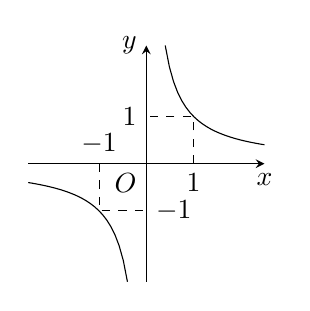
\begin{tikzpicture}[>=stealth,scale = 0.6]
    \draw [->] (-2.5,0) -- (2.5,0) node [below] {$x$};
    \draw [->] (0,-2.5) -- (0,2.5) node [left] {$y$};
    \draw (0,0) node [below left] {$O$};
    \draw [dashed] (1,0) -- (1,1) -- (0,1) (-1,0) -- (-1,-1) -- (0,-1);
    \draw (1,0) node [below] {$1$} (0,1) node [left] {$1$} (-1,0) node [above] {$-1$} (0,-1) node [right] {$-1$};
    \draw [domain = 0.4:2.5] plot (\x,{1/\x});
    \draw [domain = 0.4:2.5] plot ({-\x},{-1/\x});
\end{tikzpicture}}{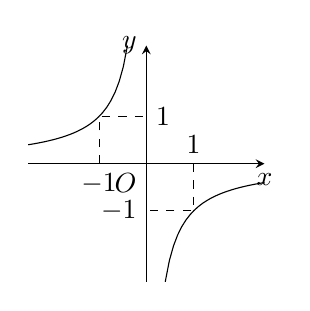
\begin{tikzpicture}[>=stealth,scale = 0.6]
    \draw [->] (-2.5,0) -- (2.5,0) node [below] {$x$};
    \draw [->] (0,-2.5) -- (0,2.5) node [left] {$y$};
    \draw (0,0) node [below left] {$O$};
    \draw [dashed] (1,0) -- (1,-1) -- (0,-1) (-1,0) -- (-1,1) -- (0,1);
    \draw (1,0) node [above] {$1$} (0,1) node [right] {$1$} (-1,0) node [below] {$-1$} (0,-1) node [left] {$-1$};
    \draw [domain = 0.4:2.5] plot (\x,{-1/\x});
    \draw [domain = 0.4:2.5] plot ({-\x},{1/\x});
\end{tikzpicture}}{\begin{tikzpicture}[>=stealth,scale = 0.6]
    \draw [->] (-2.5,0) -- (2.5,0) node [below] {$x$};
    \draw [->] (0,-2.5) -- (0,2.5) node [left] {$y$};
    \draw (0,0) node [below left] {$O$};
    \draw [dashed] (1,0) -- (1,-1) -- (0,-1);
    \draw (1,0) node [above] {$1$}  (0,-1) node [left] {$-1$};
    \draw [domain = 0.4:2.5] plot (\x,{-1/\x});
\end{tikzpicture}}{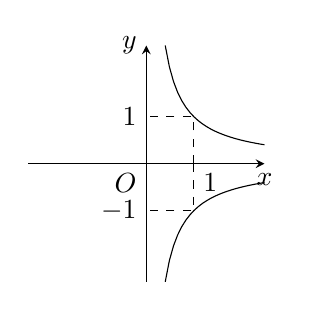
\begin{tikzpicture}[>=stealth,scale = 0.6]
    \draw [->] (-2.5,0) -- (2.5,0) node [below] {$x$};
    \draw [->] (0,-2.5) -- (0,2.5) node [left] {$y$};
    \draw (0,0) node [below left] {$O$};
    \draw [dashed] (1,0) -- (1,-1) -- (0,-1) (1,0) -- (1,1) -- (0,1);
    \draw (1,0) node [below right] {$1$} (0,1) node [left] {$1$}  (0,-1) node [left] {$-1$};
    \draw [domain = 0.4:2.5] plot (\x,{-1/\x});
    \draw [domain = 0.4:2.5] plot (\x,{1/\x});
\end{tikzpicture}}
\item 函数$y=\arctan (\sin x)$的定义域为\blank{50}, 值域为\blank{50}.
\item 函数$y=\dfrac 13\arcsin 3x+\arctan \sqrt 3x$的定义域为\blank{50}, 值域为\blank{50}.
\item 函数$y=\mathrm{arccot} \sqrt {\cos x}$的定义域为\blank{50}, 值域为\blank{50}.
\item 函数$y=\arctan \dfrac 1{x^2-1}$的定义域为\blank{50}, 值域为\blank{50}.
\item 已知方程$x^2+3\sqrt 3x+4=0$的两个实根为$x_1$与$x_2$, 记$\alpha =\arctan x_1$, $\beta =\arctan x_2$, 求$\alpha +\beta$的值.
\item 已知实数$a,b$满足$(a+1)(b+1)=2$, 求$\arctan a+\arctan b$的值.
\item 已知$|x|\le 1$, 求$\csc ^2(\arctan x)-\tan ^2(\arccos x)$的值.
\item 解方程$2\sin ^2x+3\sin x-2=0$.\\
解答在这里  原方程即$(2\sin x-1)(\sin x+2)=0$, 所以$\sin x=\dfrac 12$或$\sin x=-2$(舍去).
所以$x=k\pi +(-1)^k\dfrac{\pi }6$($k\in \mathbf{Z}$).
\item 解方程$2\sin x-\cos x=1$.\\
解答在这里  原方程即$\sin x\cdot \dfrac 2{\sqrt 5}-\cos x\cdot \dfrac 1{\sqrt 5}=\dfrac 1{\sqrt 5}$, 即$\sin (x-\varphi)=\dfrac 1{\sqrt 5}$(其中$\varphi =\arctan \dfrac 12$),
所以$x=k\pi +(-1)^k\arcsin \dfrac 1{\sqrt 5}+\arctan \dfrac 12$($k\in \mathbf{Z}$).
\item 解方程$\sin ^2x-3\sin x\cos x+1=0$.\\
解答在这里 解法一  原方程即$2\sin ^2x-3\sin x\cos x+\cos ^2x=0$.显然$\cos ^2x\ne 0$,
则有$2\tan ^2x-3\tan x+1=0$, 即$(2\tan x-1)(\tan x-1)=0$,
所以$\tan x=\dfrac 12$或$\tan x=1$, 所以$x=k\pi +\arctan \dfrac 12$或$x=k\pi +\dfrac{\pi }4$($k\in \mathbf{Z}$).
解法二  原方程即$\dfrac{1-\cos 2x}2-\dfrac 32\sin 2x+1=0$.
整理, 得$3\sin 2x+\cos 2x=3$, 于是$\sin (2x+\varphi)=\dfrac 3{\sqrt {10}}$(其中$\varphi =\arctan \dfrac 13$),
所以$2x+\varphi =k\pi +(-1)^k\arcsin \dfrac 3{\sqrt {10}}$,
故$x=\dfrac{k\pi }2+\dfrac 12(-1)^k\arcsin \dfrac 3{\sqrt {10}}-\dfrac 12\arctan \dfrac 13$($k\in \mathbf{Z}$).
\item 解方程$\tan 5x=\tan 4x$.\\
解答在这里  由已知, 得$\begin{cases} 5x\ne m\pi +\dfrac{\pi }2, \\ 4x\ne n\pi +\dfrac{\pi }2, \\ 5x=k\pi +4x \end{cases}$($m,n,k\in \mathbf{Z}$), 所以$x=k\pi$($k\in \mathbf{Z}$).
\item 解方程$\sin 2x-12(\sin x-\cos x)+12=0$.\\
解答在这里  令$\sin x-\cos x=t$($|t|\le \sqrt 2$), 则$\sin 2x=1-t^2$, 原方程可化为$1-t^2-12t+12=0$,
即$t^2+12t-13=0$, 也即$(t+13)(t-1)=0$.所以$t=-13$(舍去), 或$t=1$.
所以$\sin x-\cos x=1$, 即$\sin (x-\dfrac{\pi }4)=\dfrac{\sqrt 2}2$, 故$x=k\pi +(-1)^k\dfrac{\pi }4+\dfrac{\pi }4$($k\in \mathbf{Z}$).
\item 解方程$\sin ^2x+\sin ^22x=\sin ^23x$.\\
解答在这里  原方程即$(\sin ^23x-\sin ^2x)-\sin ^22x=0$,
所以$(\sin 3x+\sin x)(\sin 3x-\sin x)-\sin ^22x=0$, 即$4\sin 2x\cos x\cos 2x\sin x-\sin ^22x=0$,
所以$2\sin ^22x\cos 2x-\sin ^22x=0$.于是$\sin ^22x(2\cos 2x-1)=0$,
所以$\sin 2x=0$或$\cos 2x=\dfrac 12$, 故$x=\dfrac{k\pi }2$或$x=k\pi \pm \dfrac{\pi }6$($k\in \mathbf{Z}$).
\item 求实数$m$的取值范围, 使关于$x$的方程$2\sin ^2x+2\sin x\cos x-\cos ^2x-1-m=0$有解.\\
解答在这里  原方程即$\sin ^2x+2\sin x\cos x-2\cos ^2x=m$, 所以$\dfrac{1-\cos 2x}2+\sin 2x-2\cdot \dfrac{1+\cos 2x}2=m$,
即$2\sin 2x-3\cos 2x=2m+1$, 所以$\sin (2x-\varphi)=\dfrac{2m+1}{\sqrt {13}}$(其中$\varphi =\arctan \dfrac 32$).
欲使方程有解, 只需$-\sqrt {13}\le 2m+1\le \sqrt {13}$, 所以$\dfrac{-1-\sqrt {13}}2\le m\le \dfrac{-1+\sqrt {13}}2$.
\item 关于$x$的方程$\sin x+\sqrt 3\cos x+a=0$在$(0,2\pi)$内有两个相异的实数解$\alpha ,\beta$, 求实数$a$的取值及$\alpha +\beta$的值.\\
解答在这里  原方程即$\sin (x+\dfrac{\pi }3)=-\dfrac a2$.
令$y_1=\sin (x+\dfrac{\pi }3)$($0<x<2\pi$), $y_2=-\dfrac a2$.
只需$y_2$的图像(一条和$y$轴垂直的直线)和$y_1$的图像在$(0,2\pi)$内有两个交点即可.
观察下图, 得$\begin{cases} -1<-\dfrac a2<1, \\ -\dfrac a2\ne \dfrac{\sqrt 3}2, \end{cases}$即$-2<a<2$且$a\ne -\sqrt 3$.
利用中点知识, 易得$\alpha _1+\beta _1=2x_1\text=\dfrac{\pi }2$, $\alpha _2+\beta _2=2x_2\text=\dfrac 73\pi$, 即$\alpha +\beta =\dfrac{\pi }3$或$\alpha +\beta =\dfrac{7\pi }3$.
\begin{center}
    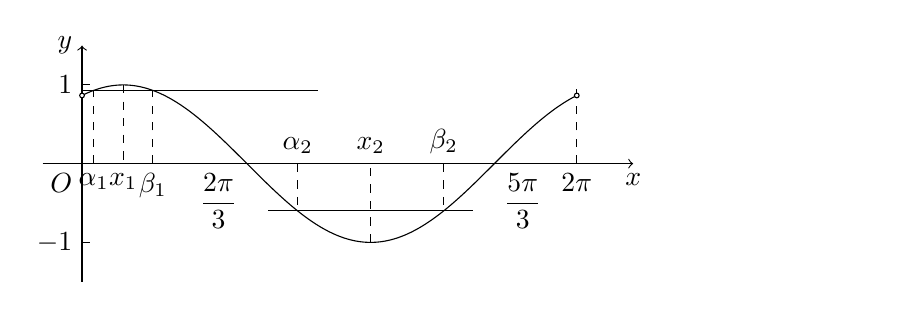
\begin{tikzpicture}
        \draw [->] (-0.5,0) -- (7,0) coordinate (X) node [below] {$x$};
        \draw [->] (0,-1.5) -- (0,1.5) node [left] {$y$};
        \draw (0,0) node [below left] {$O$} coordinate (O);
        \draw (0.1,1) -- (0,1) node [left] {$1$} (0.1,-1) -- (0,-1) node [left] {$-1$};
        \draw [domain = 0:{2*pi}, name path = curve, samples = 200] plot (\x,{(sin(\x*180/pi)+sqrt(3)*cos(\x*180/pi))/2});
        \draw [dashed] ({2*pi},0) node [below] {$2\pi$} --++ (0,1);
        \draw ({5*pi/3},0) node [below right] {$\dfrac{5\pi}3$} ({2*pi/3},0) node [below left] {$\dfrac{2\pi}3$}; 
        \path [name path = line1] (0,0.93) --++ (5,0);
        \path [name intersections = {of = line1 and curve, by = {A,B}}];
        \draw [dashed] ($(O)!(A)!(X)$) node [below] {$\alpha_1$} -- (A) ($(O)!(B)!(X)$) node [below] {$\beta_1$} -- (B);
        \draw [dashed] ({pi/6},1) -- ({pi/6},0) node [below] {$x_1$};
        \draw (0,0.93) --++ (3,0);
        \path [name path = line2] (0,-0.6) --++ (10,0);
        \path [name intersections = {of = line2 and curve, by = {C,D}}];
        \draw [dashed] ($(O)!(C)!(X)$) node [above] {$\alpha_2$} -- (C) ($(O)!(D)!(X)$) node [above] {$\beta_2$} -- (D);
        \draw ($(C)!-0.2!(D)$) -- ($(D)!-0.2!(C)$);
        \draw [dashed] ({7*pi/6},-1) -- ({7*pi/6},0) node [above] {$x_2$};
        \filldraw [fill = white, draw = black] (0,{sqrt(3)/2}) circle (0.03); 
        \filldraw [fill = white, draw = black] ({2*pi},{sqrt(3)/2}) circle (0.03);
    \end{tikzpicture}
\end{center}
\item 就实数$a$的取值范围, 讨论关于$x$的方程$\cos 2x+2\sin x+2a-3=0$在$[0,2\pi]$内解的情况.\\
解答在这里  原方程即$\sin ^2x-\sin x=a-1$, 配方, 得$(\sin x-\dfrac 12)^2=a-\dfrac 34$.
令$y_1=(\sin x-\dfrac 12)^2$, $y_2=a-\dfrac 34$.观察下图, 得:\\
(1) 当$a-\dfrac 34>\dfrac 94$或$a-\dfrac 34<0$, 即$a>3$或$a<\dfrac 34$时, 方程无解.\\
(2) 当$a-\dfrac 34=\dfrac 94$, 即$a=3$时, 方程有一解$x=\dfrac 32\pi$.\\
(3) 当$\dfrac 14<a<-\dfrac 34<\dfrac 94$或$a-\dfrac 34=0$, 即$1<a<3$或$a=\dfrac 34$时, 方程有两解.\\
(4) 当$a-\dfrac 34=\dfrac 14$, 即$a=1$时, 方程有三解: $x=0,\dfrac{\pi }2,\pi$.\\
(5) 当$0<a-\dfrac 34<\dfrac 14$, 即$\dfrac 34<a<1$时, 方程有四解.
\begin{center}
    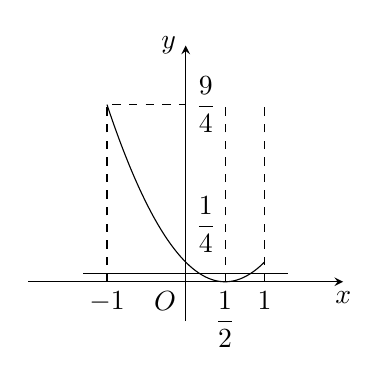
\begin{tikzpicture}[>=stealth]
        \draw [->] (-2,0) -- (2,0) node [below] {$x$};
        \draw [->] (0,-0.5) -- (0,3) node [left] {$y$};
        \draw (0,0) node [below left] {$O$};
        \draw [domain = -1:1, samples = 100] plot (\x,{(\x-0.5)^2});
        \draw [dashed] (-1,0) -- (-1,2.25) -- (0,2.25);
        \draw [dashed] (0.5,0) -- (0.5,2.25) (1,0) -- (1,2.25);
        \draw (-1,0) node [below] {$-1$} (0.5,0) node [below] {$\dfrac 12$} (1,0) node [below] {$1$};
        \draw (0,2.25) node [right] {$\dfrac 94$} (0,0.25) node [above right] {$\dfrac 14$};
        \draw (-1.3,0.1) -- (1.3,0.1);
    \end{tikzpicture}
\end{center}
\item 若关于$x$的方程$\sin x=2a-1$有解, 则$a$的取值范围是\bracket{20}.
\fourch{$0<a<1$}{$a<0$或$a>1$}{$a\le 0$或$a\ge 1$}{$0\le a\le 1$}
\item 满足$\cos (2x+45^\circ)=\sin (30^\circ -x)$的最小正角是\bracket{20}.
\fourch{$5^\circ$}{$15^\circ$}{$30^\circ$}{$37.5^\circ$}
\item 记方程$\cos 2x=1$的解集为$M$, 方程$\sin 4x=0$的解集为$P$, 则$M$与$P$的关系是\bracket{20}.
\fourch{$M\subset P$}{$M\supset P$}{$M=P$}{$M\not\subset P$且$M\not\supset P$}
\item 方程$\cos x^2=1$的解集是\bracket{20}.
\twoch{$\{x|x=2k\pi ,k\in \mathbf{Z}\}$}{$\{x|x=\pm \sqrt {2k\pi },k\in \mathbf{Z}\}$}{$\{x|x=\pm \sqrt {2k\pi },k\in \mathbf{N}\}$}{$\{x|x=\pm \sqrt {2k\pi },k\in \mathbf{N}\}\cup \{0\}$}
\item 方程$\sin ^2x=\cos ^2x$的解集是\bracket{20}.
\twoch{$\{x|x=2k\pi +\dfrac{\pi }4,k\in \mathbf{Z}\}$}{$\{x|x=k\pi +\dfrac{\pi }4,k\in \mathbf{Z}\}$}{$\{x|x=\dfrac{k\pi }2+\dfrac{\pi }4,k\in \mathbf{Z}\}$}{$\{x|x=\dfrac{k\pi }4+\dfrac{\pi }4,k\in \mathbf{Z}\}$}
I56.方程$\sqrt {1-\sin ^2x}=\sin x$的解集是\bracket{20}.
\twoch{$\{x|x=k\pi +(-1)^k\dfrac{\pi }4, \ k\in \mathbf{Z}\}$}{$\{x|x=k\pi +\dfrac{\pi }4,\ k\in \mathbf{Z}\}$}{$\{x|x=k\pi \pm \dfrac{\pi }4, \ k\in \mathbf{Z}\}$}{$\{x|x=2k\pi \pm \dfrac{\pi }4,\ k\in \mathbf{Z}\}$}
\item 方程$\tan (2x+\dfrac{\pi }3)=\dfrac{\sqrt 3}3$在$[0,2\pi)$范围内的解的个数是\bracket{20}.
\fourch{$5$}{$4$}{$3$}{$2$}
\item 若方程$2\cos x=(\dfrac 12)^a$无解, 则实数$a$的取值范围是\blank{50}.
\item 方程$\sin x=-\cos \dfrac{2\pi }5$的解集是\blank{50}.
\item 方程$\sin 2x\cdot \cot x=0$的解集是\blank{50}.
\item 若函数$f(x)=\sin (2x+5\theta)$的图像关于$y$轴对称, 则$\theta$的值等于\blank{50}.
\item 若方程$\sin x=a$在$[\dfrac{2\pi }3,\dfrac{5\pi }3]$中恰有两个不同的实数解, 则$a$的取值范围是\blank{50}.
\item 若$-6<\log _{\frac 1{\sqrt 2}}x<-2$, 求方程$\cos \pi x=1$的解集.
\item 求方程$\lg x=\cos 2x$解的个数.
\item 方程$\dfrac{\cos 2x}{1+\sin 2x}=0$的解集是\bracket{20}.
\fourch{$\{x|x=2k\pi \pm \dfrac{\pi }4, \ k\in \mathbf{Z}\}$}{$\{x|x=k\pi \pm \dfrac{\pi }4, \ k\in \mathbf{Z}\}$}{$\{x|x=k\pi +\dfrac{\pi }4, \ k\in \mathbf{Z}\}$}{$\{x|x=\dfrac{k\pi }2+\dfrac{\pi }4,\ k\in \mathbf{Z}\}$}
\item 方程$\dfrac{2\sin x}{\sin 2x}=1$在$-2\pi \le x\le 2\pi$范围内\bracket{20}.
\fourch{有一个解}{有两个解}{有三个解}{无解}
\item 下列方程中, 与方程$\sin x=\cos x$的解集相同的是\bracket{20}.
\fourch{$\sin 2x=2\sin ^2x$}{$\cos x=\sqrt {1-\cos ^2x}$}{$\sin ^2x=\cos ^2x$}{$\dfrac{\cos 2x}{\sin x+\cos x}=0$}
\item 方程$\lg _2\tan x=1+\log _2\sin x$的解集为\blank{50}.
\item 方程$\sin x+\sqrt 3\cos x=2$的解集为\blank{50}.
\item 已知$|a|\le 2$, 方程$\sin x-\sqrt 3\cos x=a$的解集为\blank{50}.
\item 方程$\cos (x+\dfrac{2\pi }3)\cos (x+\dfrac{\pi }3)=-\dfrac 14$的解集为\blank{50}.
\item 方程$\cos ^2(\dfrac{x-30^\circ }2)+\cos ^2(\dfrac{x+30^\circ }2)=1$的解集为\blank{50}.
\item 方程$\sin x\cos x+1=\sin x+\cos x$的解集为\blank{50}.
\item 方程$\sqrt 2\sin x=\sin 2x+\cos 2x$的解集为\blank{50}.
\item 方程$\sin (x-\dfrac{\pi }6)\sin (x+\dfrac{\pi }6)=\dfrac 12$的解集为\blank{50}.
\item 解方程$\sin 3x-\sin 2x+\sin x=0$.
\item 解方程$\cos 2x\cos 3x=\cos x\cos 4x$.
\item 解方程$\sin 4x\cos 3x=\sin 6x\cos x$.
\item 解方程$\sin 5x-\sin 3x=\sqrt 2\cos 4x$.
\item 解方程$\sin x+\sin 2x+\sin 3x=1+\cos x+\cos 2x$.
\item 若方程$\sin x+\cos x=m$($m\in \mathbf{R}$)在$0\le x\le \pi$范围内有两个不同的实数解, 则\bracket{20}.
\fourch{$-1\le m\le \dfrac{\sqrt 2}2$}{$-1<m\le 1$或$m=\sqrt 2$}{$1\le m<\sqrt 2$}{$-\sqrt 2<m<\sqrt 2$}
\item 方程$\sin ^2x+2\sin x-a=0$有解的条件为\bracket{20}.
\fourch{$a\in \mathbf{R}$}{$a\in [-1,3]$}{$a\in [-1,\infty)$}{$a\in (-\infty ,3]$}
\item 若方程$\cos ^2x-|\sin x|+1=0$在$-\pi <x<\pi$范围内的解之和是$p$, 解之积是$q$, 则下列结论正确的是\bracket{20}.
\twoch{$p=-1$}{$p=0$}{$q=1$}{$q=2$}
\item 设$f(x)=\cos (x-a)+\sin (x+a)$是偶函数, 求$a$的值.
\item 解方程$8\sin ^2x=3\sin 2x-1$.
\item 解方程$(\sin x+\cos x)^2=2\cos 2x$.
\item 解方程$\dfrac{1+\tan x}{1-\tan x}=1+\sin 2x$.
\item 解方程$\tan (\dfrac{\pi }3+x)+\tan (\dfrac{\pi }6-x)=\dfrac 4{\sqrt 3}$.
\item 解方程$\sin x+\cos x+\sin x\cos x=1$.
\item 解方程$\sin 2x-12(\sin x-\cos x)+12=0$.
\item 解方程$\sqrt 2(\sin x+\cos x)=\tan x+\cot x$.
\item 解方程$\sin x+\cos x+\tan x+\cot x+\sec x+\csc x+2=0$.
\item 已知方程$2x^2-4x\sin \theta +3\cos \theta =0$($0\le \theta \le \pi$)有相等的实根, 求$\theta$的值, 并解此方程.
\item 已知方程$x^2-(\sin \alpha +\cos \alpha)x+\sin ^2\alpha -\sin \alpha \cos \alpha -1=0$有两个相等的实根, 求实数$\alpha$和相成的$x$的值.
\item 已知方程$x^2-4x\cos 2\theta +2=0$和方程$2x^2+4x\sin 2\theta -1=0$有—根互为倒数, 求角$\theta$的值($0<\theta <\pi$).
\item 已知关于$x$的方程$\sin ^2x+\cos x+a=0$有解, 求实数$a$的取值范围.
\item 已知$\cos ^2x-\sin x+a=0$在$0<x\le \dfrac{\pi }2$范围内有解, 求实数$a$的取值范围.
\item 求实数$k$的取值范围, 使关于$x$的方程$\sin ^2x-\sin x+k=0$在$[-\dfrac{\pi }2,\dfrac{\pi }2]$上\\
(1) 无解;\\
(2) 恰有一解;\\
(3) 有两解.
\item (1)若关于$x$的方程$\cos 2x-\sin x+1+m=0$有解, 求实数$m$的取值范围.
I(2)若关于$x$的方程$\sin ^2x+4\sin x\cos x-2\cos ^2x=a$恒有实数解, 求实数$a$的取值范围.
\item 将$\dfrac 12,\sin \dfrac 12,\arcsin \dfrac 12$中的三个数从小到大排列.
\item 将$\dfrac 13,\cos \dfrac 13,\arccos \dfrac 13$中的三个数从小到大排列.
\item 将$\arcsin \dfrac 14,\arctan \sqrt 5,\arccos (-\dfrac 13)$中的三个数从小到大排列.
\item 已知$0<x<1$, 求证: $2\arctan \dfrac{1+x}{1-x}+\arcsin \dfrac{1-x^2}{1+x^2}=\pi$.
\item 已知$a,b,c>0$, 求证: 若$\arctan a+\arctan b+\arctan c=\pi$, 则$a+b+c=abc$, 反过来也成立.
\item 画出函数$y=\arctan x+\arctan \dfrac{1-x}{1+x}$的图像.
\item 在不同坐标系内分别画出$y=\arcsin (\sin x)(-\dfrac{\pi }2\le x\le \dfrac{3\pi }2)$和$y=\arcsin (\sin x)$($x\in \mathbf{R}$)的图像.
\item 解方程$x=\arcsin (\sin 2x)$.
\item 解方程$\cos (\pi \sin x)=\sin (\pi \cos x)$($0\le \pi <2\pi$).
\item 解方程$x^2+2x\cos (xy)+1=0$($x,y\in \mathbf{R}$).
\item 已知$\alpha ,\beta$是关于$x$的方程$a\cos x+b\sin x=c$的两个实根($a^2+b^2\ne 0$, $a\ne 2k\pi +\beta$, $k\in \mathbf{Z}$), 求证$\cos ^2\dfrac{\alpha -\beta}2=\dfrac{c^2}{a^2+b^2}$.
\item 已知$\triangle ABC$的两内角$A,B$满足方程$8\sin ^2x+3\sin 2x-4=0$, 且$A>B$, 求此三角形三边长之比.
\item 解方程$\tan (x+\dfrac{\pi }4)+\tan (x-\dfrac{\pi }4)=2\cot x$.
\item 已知关于$x$的方程$x=a\sin x+b$($0<a<1$, $b\in \mathbf{R}$)有实根, 求证: 该方程只有一个实根.
\item 已知方程$\sin ^2x+3a^2\cos x-2a^2(3a-2)-1=0$有实数解, 求实数$a$的取值范围.
\item 已知关于$x$的方程$2\cos 2x+4(a-1)\sin x-4a+1=0$在$0\le x\le 2\pi$范围内有相异两个实根, 求$a$的取值范围.
\item 已知关于$x$的方程$\cos 2x-2(2a+1)\cos x+2a^2+2a+1=0$在$[0,2\pi)$范围内有两个不同的解, 求实数$a$的取位范围.

\end{enumerate}
\end{document}